\input templates/header

\graphicspath{{figs/02/}}

\begin{document}

\title[ASD - Analisi ammortizzata]{\textbf{Algoritmi e Strutture Dati}\\[24pt]Analisi ammortizzata}

%-------------------------------------------------------------------------
\FrameTitle{}

%-------------------------------------------------------------------------
\FrameContent

%%%%%%%%%%%%%%%%%%%%%%%%%%%%%%%%%%%%%%%%%%%%%%%%%%%%%%%%%%%%%%%%%%%%%%%%%%
\section{Introduzione}

\begin{frame}{Introduzione}

\vspace{-9pt}
\begin{myboxtitle}[Analisi ammortizzata]
Una tecnica di analisi di complessità che valuta il tempo richiesto per eseguire, \alert{nel caso pessimo}, una sequenza di operazioni
su una struttura dati
\BI
\item Esistono operazioni più o meno costose.
\item Se le operazioni più costose sono poco frequenti, allora il loro\\ costo può essere \alert{ammortizzato} dalle operazioni
meno costose
\EI
\end{myboxtitle}

\bigskip
Importante differenza
\BI
\item \makebox[4cm][l]{\alert{Analisi caso medio}:}
\parbox[t]{7cm}{Probabilistica, su singola operazione}
\item \makebox[4cm][l]{\alert{Analisi ammortizzata}:}
\parbox[t]{7cm}{Deterministica, su operazioni\\ multiple, caso pessimo}
\EI

\end{frame}


\begin{frame}{Metodi per l'analisi ammortizzata}

\vspace{-9pt}
\small
\begin{myboxtitle}[Metodo dell'aggregazione]
\BI
\item Si calcola la complessità $T(n)$ per eseguire $n$ operazioni in sequenza nel \alert{caso pessimo}
\item Tecnica derivata dalla matematica
\EI
\end{myboxtitle}
\begin{myboxtitle}[Metodo degli accantonamenti]
\BI
\item Alle operazioni vengono assegnati \alert{costi ammortizzati} che possono essere maggiori/minori del loro costo effettivo
\item Tecnica derivata dall'economia
\EI
\end{myboxtitle}
\begin{myboxtitle}[Metodo del potenziale]
\BI
\item Lo stato del sistema viene descritto con una \alert{funzione di potenziale}
\item Tecnica derivata dalla fisica	
\EI
\end{myboxtitle}

\end{frame}


\section{Contatore binario}	

\begin{frame}[shrink=10]{Esempio -- Contatore binario}

\vspace{-9pt}
\begin{myboxtitle}[Contatore binario]
\BI
\item Contatore binario di $k$ bit con un vettore $A$ di booleani 0/1
\item Bit meno significativo in $A[0]$, bit più significativo in $A[k-1]$
\item Valore del contatore: \parbox[c]{6cm}{{ \[x = \sum_{i=0}^{k-1} A[i] \cdot 2^i\]}}
\vspace{-4pt}
\item Operazione \textsf{increment}() che incrementa il contatore di $1$
\EI
\end{myboxtitle}

\smallskip
\begin{Procedure}
\caption[A]{\textsf{increment}($\INTARRAY\ A$, \INTEGER $k$)}
\INTEGER $i = 0$\;
\While{$i < k$ \AND $A[i] \Eq 1$}{
  $A[i] = 0$\;
  $i = i+1$\;
}
\If{$i < k$}{
  $A[i] = 1$\;
}
\end{Procedure}

\end{frame}


\begin{frame}{Esempio}
	
\vspace{-6pt}
\small
\begin{tabular}{ccccccccc}
 $x$  &  $A[7]$ & $A[6]$ & $A[5]$ & $A[4]$ & $A[3]$ & $A[2]$ & $A[1]$ & $A[0]$ \\\hline
 0 & 0 & 0 & 0 & 0 & 0 & 0 & 0 & 0 \\
 1 & 0 & 0 & 0 & 0 & 0 & 0 & 0 & 1 \\
 2 & 0 & 0 & 0 & 0 & 0 & 0 & 1 & 0 \\
 3 & 0 & 0 & 0 & 0 & 0 & 0 & 1 & 1 \\
 4 & 0 & 0 & 0 & 0 & 0 & 1 & 0 & 0 \\
 5 & 0 & 0 & 0 & 0 & 0 & 1 & 0 & 1 \\
 6 & 0 & 0 & 0 & 0 & 0 & 1 & 1 & 0 \\
 7 & 0 & 0 & 0 & 0 & 0 & 1 & 1 & 1 \\
 8 & 0 & 0 & 0 & 0 & 1 & 0 & 0 & 0 \\
 9 & 0 & 0 & 0 & 0 & 1 & 0 & 0 & 1 \\
10 & 0 & 0 & 0 & 0 & 1 & 0 & 1 & 0 \\
11 & 0 & 0 & 0 & 0 & 1 & 0 & 1 & 1 \\
12 & 0 & 0 & 0 & 0 & 1 & 1 & 0 & 0 \\
13 & 0 & 0 & 0 & 0 & 1 & 1 & 0 & 1 \\
14 & 0 & 0 & 0 & 0 & 1 & 1 & 1 & 0 \\
15 & 0 & 0 & 0 & 0 & 1 & 1 & 1 & 1 \\
16 & 0 & 0 & 0 & 1 & 0 & 0 & 0 & 0 \\
\end{tabular}    

\end{frame}	



\subsection{Aggregazione}

\begin{frame}{Analisi ammortizzata -- Metodo dell'aggregazione}

\vspace{-9pt}
\begin{myboxtitle}[Metodo dell'aggregazione]
\BI
\item Si calcola la complessità $T(n)$ per eseguire \alert{$n$ operazioni} in \alert{sequenza} nel \alert{caso pessimo}
\item Si calcola il \alert{costo ammortizzato $T(n)/n$ } come \alert{media} su $n$ operazioni
\EI
\end{myboxtitle}

\BB{
\BIL
\item \alert{Sequenza}: si considera l'evoluzione della struttura dati data una sequenza di operazioni 
\item \alert{Caso pessimo}: si considera la peggior sequenza di operazioni
\item \alert{Aggregazione}: sommatoria delle complessità individuali
\EIL
}


\end{frame}

\begin{frame}{Analisi ammortizzata -- Metodo dell'aggregazione}

\BB{
\BIL
\item Qual è il costo $T(n)$ per eseguire $n$ operazioni (caso pessimo)?
\item Qual è il costo ammortizzato $T(n)/n$?
\EIL
}

\bigskip
\begin{overprint}
\onslide<1|handout:0>
\begin{Procedure}
\caption[A]{\textsf{increment}($\INTARRAY\ A$, \INTEGER $k$)}
\INTEGER $i = 0$\;
\While{$i < k$ \AND $A[i] \Eq 1$}{
  $A[i] = 0$\;
  $i = i+1$\;
}
\If{$i < k$}{
  $A[i] = 1$\;
}
\end{Procedure}
\onslide<2|handout:1>
\begin{myboxtitle}[Analisi “grossolana”]
\BIL
\item Sono necessari \alert{$k = \lceil \log (n+1) \rceil$} bit per rappresentare $n$
\item Una chiamata \textsf{increment}() richiede tempo $O(k)$ nel caso pessimo 
\item Costo di $n$ operazioni: \alert{$T(n) = O(nk)$}
\item Costo di $1$ operazione: \alert{$T(n)/n = O(k) = O(\log n)$}
\EIL
\end{myboxtitle}
\onslide<3|handout:2>
\TwoColsCustom{0.65}{0.33}{
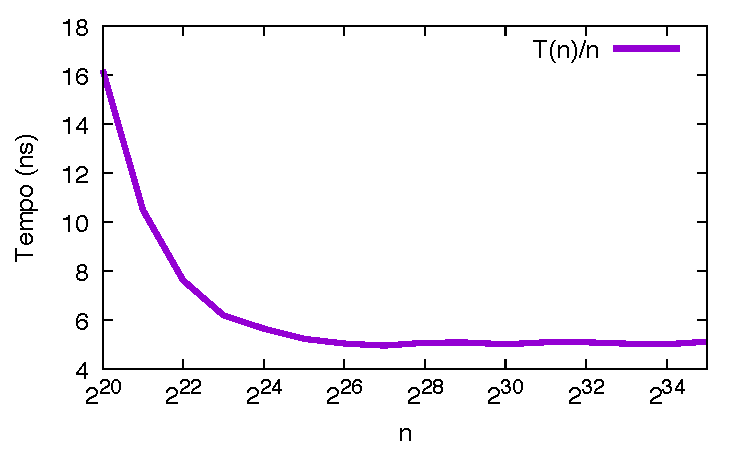
\includegraphics[width=\textwidth]{plot1.pdf}
}{
\BIL
\item $n=2^k$ operazioni
\item $k \in [20,35]$
\item Eseguito in Java
\EIL
}
\end{overprint}

\end{frame}

\begin{frame}{Quanto costano $n$ operazioni di incremento?}

\vspace{-9pt}
\begin{myboxtitle}[Considerazioni per un'analisi più stretta]
\BI
\item Possiamo osservare che il tempo necessario ad eseguire l’intera sequenza è proporzionale al numero di bit che vengono modificati
\item Quanti bit vengono modificati?
\EI
\end{myboxtitle}

\end{frame}

\begin{frame}{Esempio}
	
\vspace{-6pt}
\small
\begin{tabular}{ccccccccc|c}
 $x$  &  $A[7]$ & $A[6]$ & $A[5]$ & $A[4]$ & $A[3]$ & $A[2]$ & $A[1]$ & $A[0]$ & \#bit \\\hline
 0 & 0 & 0 & 0 & 0 & 0 & 0 & 0 & 0 \\
 1 & 0 & 0 & 0 & 0 & 0 & 0 & 0 & \alert{1} & 1 \\
 2 & 0 & 0 & 0 & 0 & 0 & 0 & \alert{1} & \alert{0} & 2 \\
 3 & 0 & 0 & 0 & 0 & 0 & 0 & 1 & \alert{1} & 1 \\
 4 & 0 & 0 & 0 & 0 & 0 & \alert{1} & \alert{0} & \alert{0} & 3 \\
 5 & 0 & 0 & 0 & 0 & 0 & 1 & 0 & \alert{1} & 1 \\
 6 & 0 & 0 & 0 & 0 & 0 & 1 & \alert{1} & \alert{0} & 2 \\
 7 & 0 & 0 & 0 & 0 & 0 & 1 & 1 & \alert{1} & 1 \\
 8 & 0 & 0 & 0 & 0 & \alert{1} & \alert{0} & \alert{0} & \alert{0} & 4 \\
 9 & 0 & 0 & 0 & 0 & 1 & 0 & 0 & \alert{1} & 1 \\
10 & 0 & 0 & 0 & 0 & 1 & 0 & \alert{1} & \alert{0} & 2 \\
11 & 0 & 0 & 0 & 0 & 1 & 0 & 1 & \alert{1} & 1 \\
12 & 0 & 0 & 0 & 0 & 1 & \alert{1} & \alert{0} & \alert{0} & 3 \\
13 & 0 & 0 & 0 & 0 & 1 & 1 & 0 & \alert{1} & 1 \\
14 & 0 & 0 & 0 & 0 & 1 & 1 & \alert{1} & \alert{0} & 2 \\
15 & 0 & 0 & 0 & 0 & 1 & 1 & 1 & \alert{1} & 1 \\
16 & 0 & 0 & 0 & \alert{1} & \alert{0} & \alert{0} & \alert{0} & \alert{0} & 5 \\
\end{tabular}    
    
\end{frame}	

\begin{frame}[shrink=5]{Esempio}

\vspace{-6pt}
\small
\begin{tabular}{ccccccccc|c}
 $x$  &  $A[7]$ & $A[6]$ & $A[5]$ & $A[4]$ & $A[3]$ & $A[2]$ & $A[1]$ & $A[0]$ & \#bit \\\hline
 0 & 0 & 0 & 0 & 0 & 0 & 0 & 0 & 0 \\
 1 & 0 & 0 & 0 & 0 & 0 & 0 & 0 & \alert{1} & 1 \\
 2 & 0 & 0 & 0 & 0 & 0 & 0 & \alert{1} & \alert{0} & 2 \\
 3 & 0 & 0 & 0 & 0 & 0 & 0 & 1 & \alert{1} & 1 \\
 4 & 0 & 0 & 0 & 0 & 0 & \alert{1} & \alert{0} & \alert{0} & 3 \\
 5 & 0 & 0 & 0 & 0 & 0 & 1 & 0 & \alert{1} & 1 \\
 6 & 0 & 0 & 0 & 0 & 0 & 1 & \alert{1} & \alert{0} & 2 \\
 7 & 0 & 0 & 0 & 0 & 0 & 1 & 1 & \alert{1} & 1 \\
 8 & 0 & 0 & 0 & 0 & \alert{1} & \alert{0} & \alert{0} & \alert{0} & 4 \\
 9 & 0 & 0 & 0 & 0 & 1 & 0 & 0 & \alert{1} & 1 \\
10 & 0 & 0 & 0 & 0 & 1 & 0 & \alert{1} & \alert{0} & 2 \\
11 & 0 & 0 & 0 & 0 & 1 & 0 & 1 & \alert{1} & 1 \\
12 & 0 & 0 & 0 & 0 & 1 & \alert{1} & \alert{0} & \alert{0} & 3 \\
13 & 0 & 0 & 0 & 0 & 1 & 1 & 0 & \alert{1} & 1 \\
14 & 0 & 0 & 0 & 0 & 1 & 1 & \alert{1} & \alert{0} & 2 \\
15 & 0 & 0 & 0 & 0 & 1 & 1 & 1 & \alert{1} & 1 \\
16 & 0 & 0 & 0 & \alert{1} & \alert{0} & \alert{0} & \alert{0} & \alert{0} & 5 \\\hline
\#bit & 0 & 0 & 0 & 1 & 2 & 4 & 8 & 16 &  \\
\end{tabular}    

\end{frame}


\begin{frame}{Contatore binario -- Metodo dell'aggregazione}	
Dalla simulazione si vede che:
\BI
\item $A[0]$ viene modificato ogni $1$ incremento
\item $A[1]$ viene modificato ogni $2$ incrementi
\item $A[2]$ viene modificato ogni $4$ incrementi
\item \ldots
\item $A[i]$ viene modificato ogni $2^i$ incrementi
\EI
\begin{myboxtitle}[Analisi ammortizzata]
\BIL
\item \alert{Costo totale}:
$\displaystyle
T(n) = \sum_{i=0}^{k-1} \left\lfloor \frac{n}{2^i} \right\rfloor \leq n \sum_{i=0}^{k-1}  \frac{1}{2^i} \leq n \sum_{i=0}^{+\infty}  \left(\frac{1}{2}\right)^i = 2n
$
\item \alert{Costo ammortizzato}: $T(n)/n \leq 2n/n = 2  = O(1)$
\EIL
\end{myboxtitle}
\end{frame}

\subsection{Ammortamento}

\begin{frame}{Analisi ammortizzata -- Metodo degli accantonamenti}
\BI
\item Si assegna un costo ammortizzato \emph{potenzialmente} distinto ad ognuna delle operazioni possibili
\item Il costo ammortizzato può essere diverso dal costo effettivo
\BI
\item Le operazioni meno costose vengono caricate di un costo aggiuntivo detto \alert{credito}
\[
\alert{\mathit{costo\ ammortizzato} = \mathit{costo\ effettivo} + \mathit{credito\ prodotto}}
\]
\item I crediti accumulati sono usati per pagare le operazioni più costose
\[
\alert{\mathit{costo\ ammortizzato} = \mathit{costo\ effettivo} - \mathit{credito\ consumato}}
\]
\EI
\EI
\end{frame}


\begin{frame}{Analisi ammortizzata -- Metodo degli accantonamenti}

\vspace{-9pt}
\begin{myboxtitle}[Obiettivi]
\BI
\item Dimostrare che la somma dei costi ammortizzati $a_i$ è un limite superiore ai costi effettivi $c_i$:
\[
 \sum_{i=1}^n c_i \leq \sum_{i=1}^n a_i
\]
\item Dimostrare che il valore così ottenuto è “poco costoso”
\EI
\end{myboxtitle}

\bigskip
Alcuni punti da ricordare:
\BI
\item La dimostrazione deve valere per tutte le sequenze (caso pessimo)
\item Il credito dopo l'operazione $t$-esima è espresso dalla seguente formula ed è sempre positivo
\EI
\[
 \sum_{i=1}^t a_i - \sum_{i=1}^t c_i \geq 0
\]

\end{frame}

\begin{frame}{Contatore binario  -- Metodo degli accantonamenti}

\BI
\item Costo effettivo dell'operazione \textsf{increment}(): \alert{$d$} \\
\BI
  \item Dove $d$ è il numero di bit che cambiano valore
\EI
\item Costo ammortizzato dell'operazione \textsf{increment}(): \alert{$2$}
\BI 
  \item $1$ per cambio di un bit da $0$ a $1$ (costo effettivo)
  \item $1$ per il futuro cambio dello stesso bit da $1$ a $0$
\EI
\item  Ne consegue che: 
\BI
\item In ogni istante, il credito è pari al numero di bit $1$  presenti
\item Costo totale: $O(n)$
\item Costo ammortizzato: $O(1)$
\EI
\EI
\end{frame}

\subsection{Potenziale}

\begin{frame}{Analisi ammortizzata -- Metodo del potenziale}

\vspace{-9pt}
\begin{myboxtitle}[Funzione di potenziale]
\BIL
\item Una \alert{funzione di potenziale $\Phi$} associa ad uno \alert{stato $S$} della struttura dati la \alert{"quantità di lavoro" $\Phi(S)$} che è stato contabilizzato nell'analisi ammortizzata, ma non ancora eseguito
\item In altre parole, $\Phi(S)$ rappresenta la quantità di energia potenziale "immagazzinata" in quello stato
\EIL
\end{myboxtitle}

\begin{myboxtitle}[Costo ammortizzato]
\alert{Costo ammortizzato} = \alert{Costo effettivo} + \alert{Variazione di potenziale}.

\[
  a_i = c_i + \Phi(S_i) - \Phi(S_{i-1})
\]
dove $S_i$ è lo stato associato alla $i$-esima operazione.
\end{myboxtitle}

\end{frame}

\begin{frame}{Analisi ammortizzata -- Metodo del potenziale}

\vspace{-3pt}
\BB{Costo ammortizzato,  sequenza di $n$ operazioni}
\begin{align*}
  A &= \sum_{i=1}^n a_i \\
    &= \sum_{i=1}^n \left(c_i + \Phi(S_i) - \Phi(S_{i-1}) \right) \\
    &= \sum_{i=1}^n c_i + \sum_{i=1}^n \left(\Phi(S_i) - \Phi(S_{i-1}) \right) \\
    &= C + \Phi(S_1) - \Phi(S_0) + \Phi(S_2) - \Phi(S_1) + \ldots + \Phi(S_n) - \Phi(S_{n-1}) \\
    &= C + \Phi(S_n) - \Phi(S_0)
\end{align*}

\vspace{-6pt}
Se la variazione di potenziale $\Phi(S_n) - \Phi(S_0)$ è non negativa,\\
\alert{il costo ammortizzato $A$ è un limite superiore al costo reale}
\end{frame}

\begin{frame}{Contatore binario -- Metodo del potenziale}
\BIL
\item Scegliamo come funzione potenziale $\Phi$ il numero bit $1$ presenti nel contatore
\item Operazione \textsf{increment}():
\BI
  \item $t$ è il numero di bit $1$ incontrati a partire dal meno significativo, prima di incontrare un bit $0$
  \item \makebox[4cm][l]{\alert{Costo effettivo}:} $1+t$
  \item \makebox[4cm][l]{\alert{Variazione di potenziale}:} $1-t$
  \item \makebox[4cm][l]{\alert{Costo ammortizzato}:} $1+t + 1 -t = 2$
\EI
\item All'inizio, zero bit accesi $\Rightarrow$ $\Phi(S_0)  = 0$ 
\item Alla fine, $\Phi(S_n) \geq 0$  $\Rightarrow$ la differenza di potenziale è non negativa
\EIL

\end{frame}

\section{Vettori dinamici}

\subsection{Inserimento}

\begin{frame}{Vettori dinamici -- Espansione}

\vspace{-9pt}
\begin{myboxtitle}[Sequenze implementate tramite \alert{vettori dinamici}]
\BI
\item Si alloca un vettore di una certa dimensione detta \alert{capacità}
\item L'inserimento di un elemento “in mezzo”  ha costo $O(n)$
\item Inserire un elemento “in fondo” alla sequenza (\alert{append}) ha costo $O(1)$
\EI
\end{myboxtitle}

\begin{overprint}
\onslide<1|handout:1>\centerline{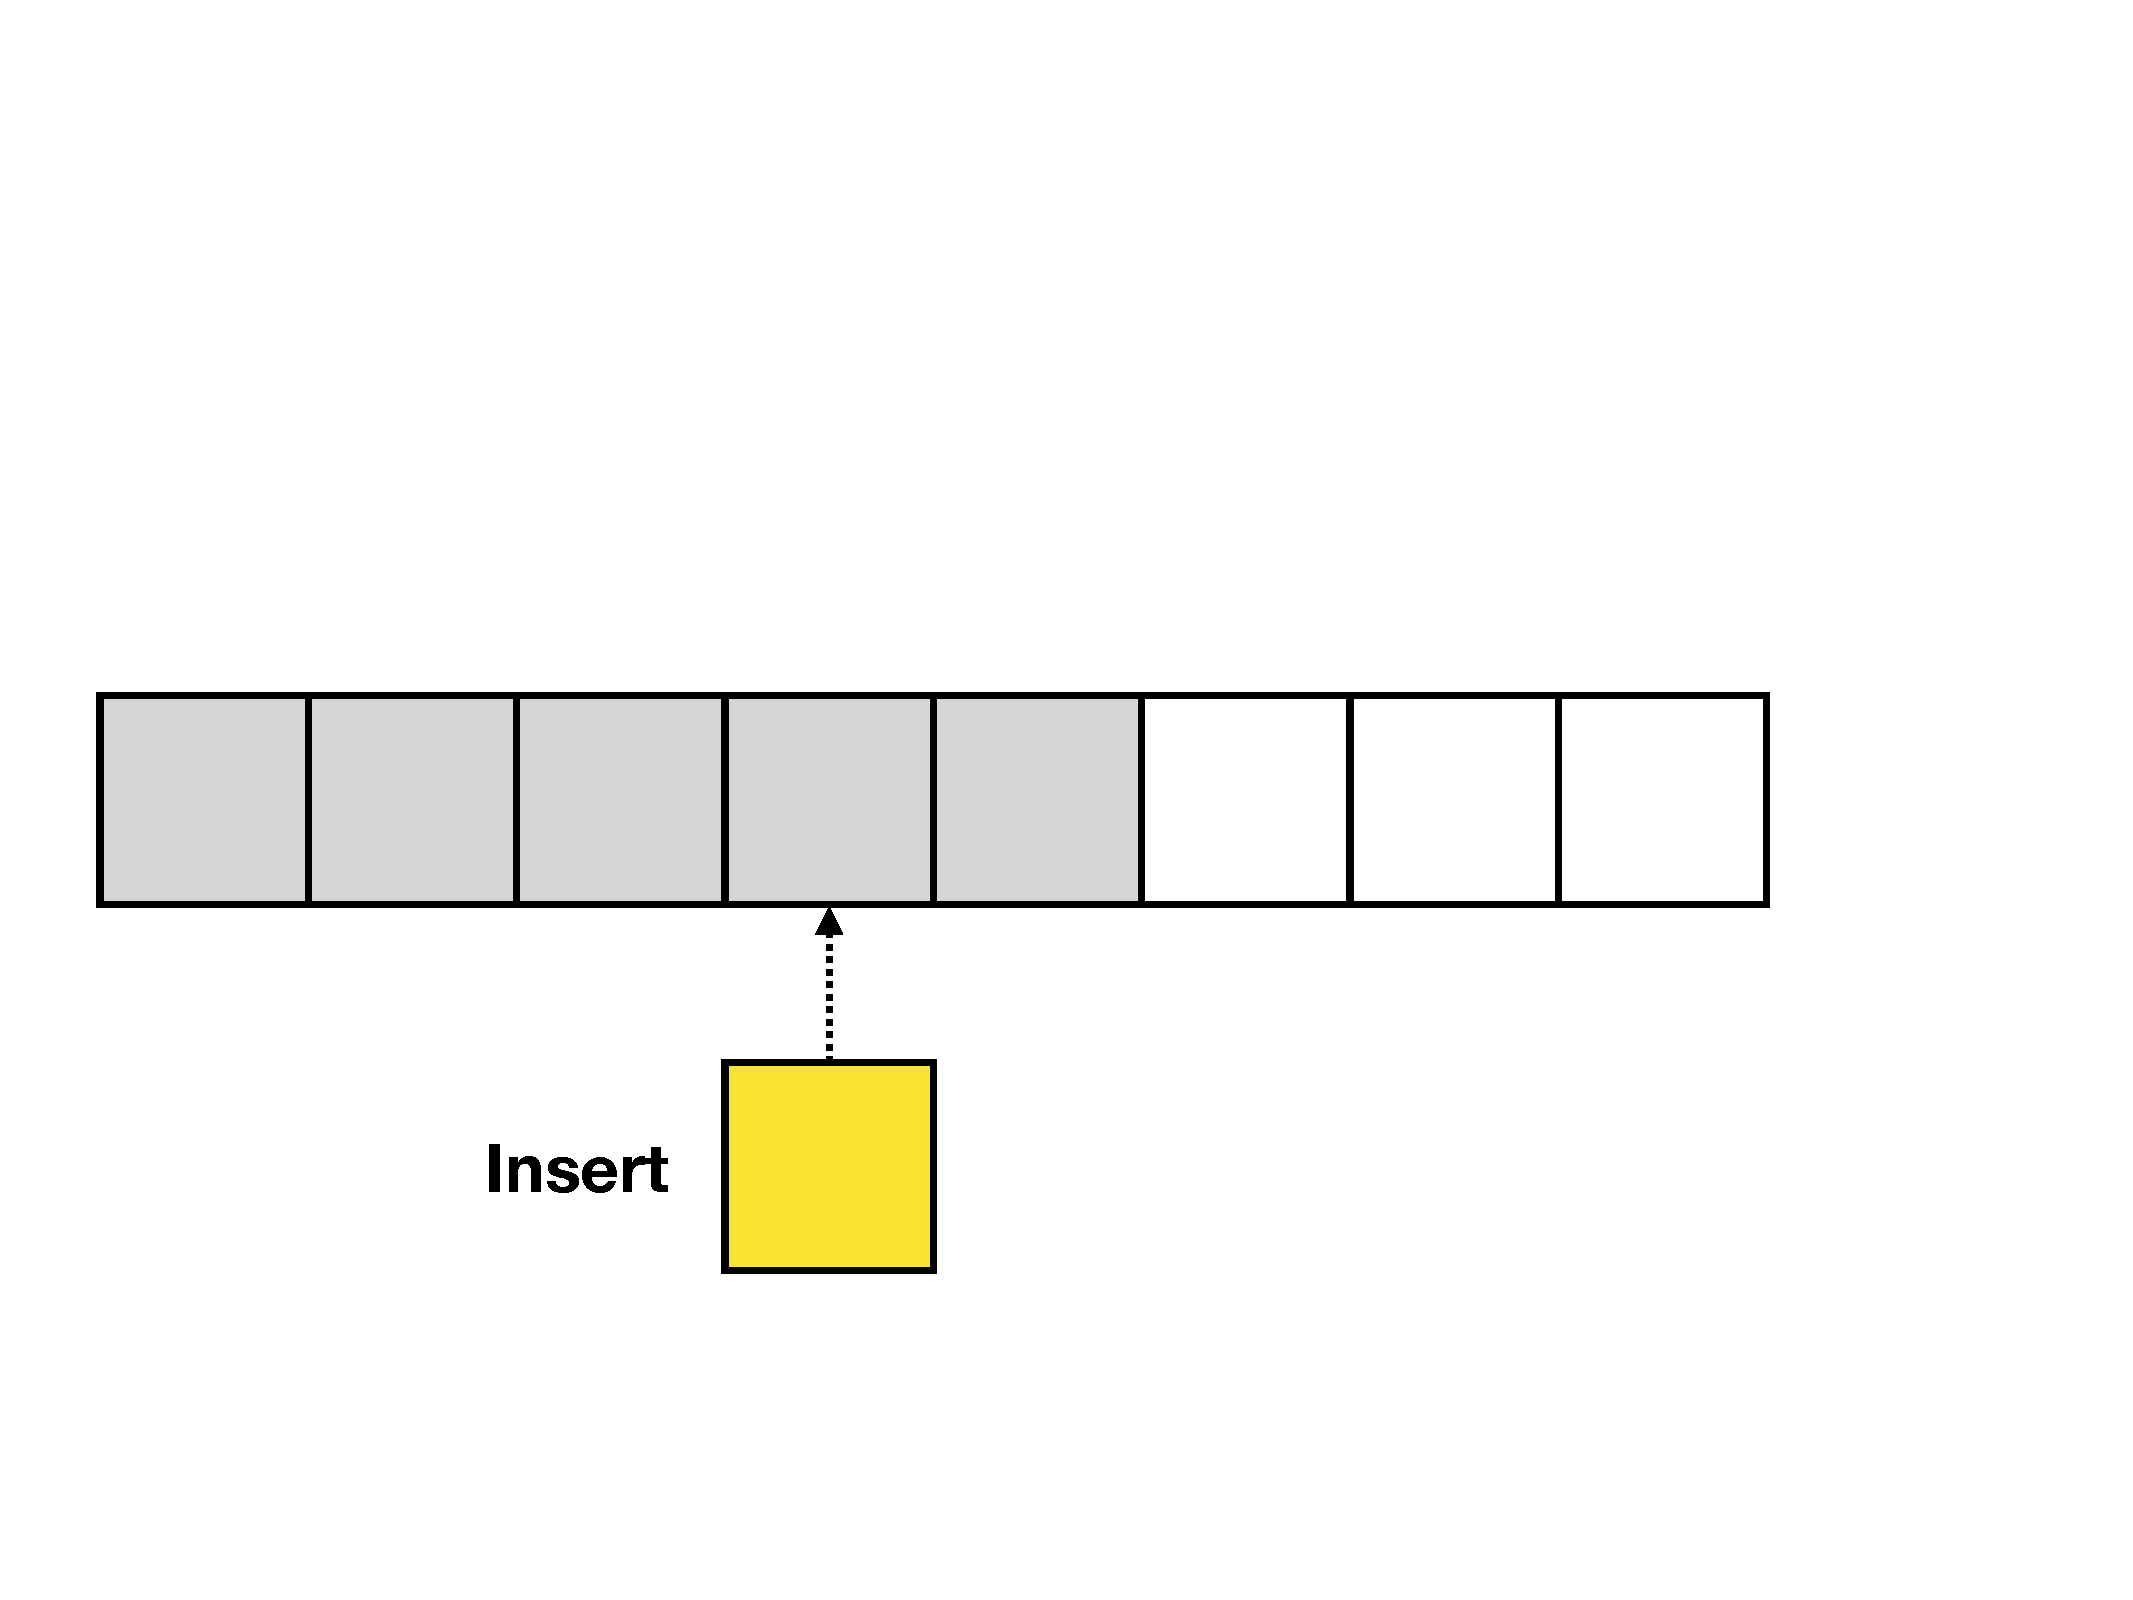
\includegraphics[width=0.8\textwidth,page=1]{append-insert.pdf}}
\onslide<2|handout:2>\centerline{\includegraphics[width=0.8\textwidth,page=2]{append-insert.pdf}}
\onslide<3|handout:3>\centerline{\includegraphics[width=0.8\textwidth,page=3]{append-insert.pdf}}
\onslide<4|handout:4>\centerline{\includegraphics[width=0.8\textwidth,page=4]{append-insert.pdf}}
\onslide<5|handout:5>\centerline{\includegraphics[width=0.8\textwidth,page=5]{append-insert.pdf}}
\end{overprint}

\end{frame}

\begin{frame}{Vettori dinamici -- Espansione}


\vspace{-9pt}
\begin{myboxtitle}[Problema]
\BI
\item Non è noto a priori quanti elementi entreranno nella sequenza
\item La capacità selezionata può rivelarsi insufficiente.
\EI
\end{myboxtitle}

\begin{myboxtitle}[Soluzione]
\BI
\item Si alloca un vettore di capacità maggiore, si ricopia il contenuto del vecchio vettore nel nuovo e si rilascia il vecchio vettore
\item Esempi: \texttt{java.util.Vector}, \texttt{java.util.ArrayList}
\EI
\end{myboxtitle}


\end{frame}

\begin{frame}[fragile,shrink]{Vettori dinamici in Java}

\begin{lstlisting}[language=java]
private Object[] buffer = new Object[INITSIZE];

<@\textcolor{blue}{// Raddoppiamento}@>
private void <@\textcolor{blue}{doubleStorage}@>() {
  Object[] newb = new Object[<@\textcolor{blue}{2*buffer.length}@>];
  System.arraycopy(buffer,0, newb,0, buffer.length);
  buffer = newb;
}

<@\textcolor{blue}{// Incremento fisso}@>
private void <@\textcolor{blue}{incrementStorage}()@> {
  Object[] newb = new Object[<@\textcolor{blue}{buffer.length+INCREMENT}@>];
  System.arraycopy(buffer,0, newb,0, buffer.length);
  buffer = newb;
}
\end{lstlisting}
	
\end{frame}



\begin{frame}[fragile]{Vettori dinamici -- Espansione}

\vspace{-9pt}
\onslide<1-2|handout:1>
\begin{myboxtitle}[Domanda]
Qual è il migliore fra i due?
\BI
\item Raddoppiamento
\item Incremento costante
\EI
\end{myboxtitle}

\onslide<2|handout:1>
\begin{myboxtitle}[Dalla documentazione Java: ArrayList.add():]
\begin{alltt}
As elements are added to an \alert{ArrayList}, its capacity grows 
automatically. The details of the growth policy are not 
specified beyond the fact that adding an element has 
\alert{constant} amortized time cost.
\end{alltt}
\end{myboxtitle}


\end{frame}

\begin{frame}[fragile,shrink]{Vettori dinamici in Java -- Quale approccio?}

\vspace{-9pt}
\begin{lstlisting}[language=java]
private Object[] buffer = new Object[INITSIZE];

<@\textcolor{blue}{// Raddoppiamento -- Utilizzato in ArrayList (1.2)}@>
private void <@\textcolor{blue}{doubleStorage}@>() {
  Object[] newb = new Object[<@\textcolor{blue}{2*buffer.length}@>];
  System.arraycopy(buffer,0, newb,0, buffer.length);
  buffer = newb;
}

<@\textcolor{blue}{// Incremento fisso -- Utilizzato in Vector (1.0)}@>
private void <@\textcolor{blue}{incrementStorage}()@> {
  Object[] newb = new Object[<@\textcolor{blue}{buffer.length+INCREMENT}@>];
  System.arraycopy(buffer,0, newb,0, buffer.length);
  buffer = newb;
}
\end{lstlisting}

\end{frame}


\begin{frame}{Analisi ammortizzata, raddoppiamento del vettore}

\vspace{-9pt}
\begin{columns}[T]
\begin{column}{0.6\textwidth}
\alert{Costo effettivo di un'operazione \textsf{add}()}:
\[
c_i = \begin{cases} 
     i & \textrm{$\exists k \in \mathbb{Z}^{+}_0: i=2^k+1$}\\
     1 & \textrm{altrimenti}
  \end{cases}
\]

\bigskip
Assunzioni:
\BI
\item Dimensione iniziale: 1
\item Costo di scrittura di un elemento: 1
\EI

\end{column}
\hfill
\begin{column}{0.30\textwidth}
{\footnotesize
\begin{tabular}{|r|l|}
\hline
$n$ & costo \\
\hline
$1$ & $1$ \\
$2$ & $1 + 2^0 = 2$ \\
$3$ & $1 + 2^1 = 3$ \\
$4$ & $1$ \\
$5$ & $1 + 2^2 = 5$\\
$6$ & $1$ \\
$7$ & $1$ \\
$8$ & $1$ \\
$9$ & $1 + 2^3 = 9$ \\
$10$ & $1$ \\
$11$ & $1$ \\
$12$ & $1$ \\
$13$ & $1$ \\
$14$ & $1$ \\
$15$ & $1$ \\
$16$ & $1$ \\
$17$ & $1 + 2^4 = 17$ \\
\hline
\end{tabular}
}
\end{column}
\end{columns}


\end{frame}

\begin{frame}{Analisi ammortizzata, raddoppiamento del vettore}
	
\vspace{-9pt}
\begin{columns}[T]
\begin{column}{0.57\textwidth}
\alert{Costo effettivo di $n$ operazioni \textsf{add}()}:
\begin{align*}
  T(n) &= \sum_{i=1}^n c_i \\
       &= n + \sum_{j=0}^{\lfloor \log n \rfloor} 2^j \\
	   &=  n + 2^{\lfloor \log n \rfloor + 1} - 1 \\
	   &\leq  n + 2^{\log n + 1} - 1 \\
	   &=  n + 2n - 1 = \alert{O(n)}
\end{align*}
\end{column}
\begin{column}{0.43\textwidth}
\alert{Costo ammortizzato di un'operazione \textsf{add}()}: \[ T(n)/n = \frac{O(n)}{n} = O(1)\]
\end{column}
\end{columns}

\end{frame}

\begin{frame}{Analisi ammortizzata, incremento del vettore}

\vspace{-9pt}
\begin{columns}[T]
\begin{column}{0.6\textwidth}
\alert{Costo effettivo di un'operazione \textsf{add}()}:

\[
c_i = \begin{cases} 
     i & \textrm{$(i \bmod d) = 1$}\\
     1 & \textrm{altrimenti}
  \end{cases}
\]

\bigskip
Assunzioni:
\BI
\item Incremento: $d$
\item Dimensione iniziale: $d$
\item Costo di scrittura di un elemento: 1
\EI

\bigskip
Nell'esempio:
\BI
\item $d=4$
\EI



\end{column}
\hfill
\begin{column}{0.30\textwidth}
{\footnotesize
\begin{tabular}{|r|l|}
\hline
$n$ & costo \\
\hline
$1$ & $1$ \\
$2$ & $1$ \\
$3$ & $1$ \\
$4$ & $1$ \\
$5$ & $1 + d = 5$\\
$6$ & $1$ \\
$7$ & $1$ \\
$8$ & $1$ \\
$9$ & $1 + 2d = 9$ \\
$10$ & $1$ \\
$11$ & $1$ \\
$12$ & $1$ \\
$13$ & $1 + 3d = 13$ \\
$14$ & $1$ \\
$15$ & $1$ \\
$16$ & $1$ \\
$17$ & $1 + 4d = 17$ \\
\hline
\end{tabular}
}
\end{column}
\end{columns}

\end{frame}

\begin{frame}{Analisi ammortizzata, incremento del vettore}
	
\vspace{-9pt}
\begin{columns}[T]
\begin{column}{0.57\textwidth}
\alert{Costo effettivo di $n$ operazioni \textsf{add}()}:
\begin{align*}
  T(n) &= \sum_{i=1}^{n} c_i \\
    &= n + \sum_{j=1}^{\lfloor n/d \rfloor} d \cdot j \\
    &= n + d\sum_{j=1}^{\lfloor n/d \rfloor} j \\
    &= n + d \frac{(\lfloor n/d \rfloor+1)\lfloor n/d \rfloor}{2} \\
    &\leq n + \frac{(n/d+1)n}{2} =  \alert{O(n^2)}
\end{align*}
\end{column}
\begin{column}{0.43\textwidth}
\alert{Costo ammortizzato di un'operazione \textsf{add}()}: \[ T(n)/n = \frac{O(n^2)}{n} = O(n)\]
\end{column}
\end{columns}

\end{frame}

\begin{frame}{Reality check}

\begin{center}
\begin{tabular}{|r|r|r|}
\hline
\textbf{Linguaggio} & \textbf{Struttura dati} & \textbf{Fattore espansione} \\
\hline
GNU C++ & \texttt{std::vector} & 2.0 \\
\hline
Microsoft VC++ 2003 & \texttt{vector} & 1.5 \\
\hline
C\# & \texttt{List} & 2.0 \\
\hline
Python & \texttt{list} & 1.125 \\
\hline
Oracle Java & \texttt{ArrayList} & 2.0 \\
\hline
OpenSDK Java & \texttt{ArrayList} & 1.5 \\
\hline
\end{tabular}
\end{center}

\end{frame}

\begin{frame}{Non ancora convinti? Allocazione memoria}

\vspace{-9pt}
\begin{myboxtitle}[Domande]
\BI
\item Quanto memoria occupa un intero 32 bit se memorizzato in un \alert{vettore dinamico}, nel caso pessimo/ottimo?
\item Quanto memoria occupa un intero 32 bit se memorizzato in un \alert{elemento di una lista}, nel caso pessimo/ottimo? 
\EI
\end{myboxtitle}

\begin{overprint}
\onslide<1|handout:0>
\onslide<2|handout:1>
\begin{myboxtitle}[Vettori]
\BIL
\item Nel caso ottimo (vettore pieno): \alert{$4n$ byte}
\item Nel caso pessimo (vettore appena raddoppiato): \alert{$2 \cdot 4n$ byte}
\EIL
\end{myboxtitle}
\onslide<3|handout:2>
\begin{myboxtitle}[Liste]
Alcuni dati interessanti (e inquietanti) relativi a Java:
\BIL
\item un \texttt{Object} vuoto richiede 16 byte in un'architettura a 64 bit
\item l'allocazione di memoria avviene per multipli di 8 byte
\item un oggetto contenente un intero e due reference (lista bidirezionale) richiede 32-40 byte
(Java compressed references)
\EIL
\end{myboxtitle}
\end{overprint}

\end{frame}

\begin{frame}[fragile,shrink]{Non ancora convinti? String vs StringBuffer}

\begin{alltt}
public static void print(int dim)
\{
  StringBuffer buffer = new \alert{StringBuffer}();
  for (int i=0; i < dim; i++) \{
    \alert{buffer.append('x')};	
  \}

  String string = new \alert{String}();
  for (int i=0; i < dim; i++) \{
    \alert{string = string + 'x'};	
  \} 
\}
\end{alltt}

\end{frame}

\begin{frame}{Non ancora soddisfatti? String vs StringBuffer}

\begin{center}
\begin{tabular}{|r|r|r|}
\hline
\texttt{dim} & \texttt{StringBuffer} (ms) & \texttt{\ \ \ \ \ \ String} (ms)\\
\hline
1024 & 0 & 3 \\
2048 & 1 & 7 \\  
4096 & 1 & 13 \\
8192 & 1 & 22 \\
16384 & 3 & 71 \\
32768 & 4 & 285 \\
65536 & 3 & 1130 \\
131072 & 4 & 4847 \\
262144 & 6 & 20853 \\
524288 & 11 & 84982 \\
1048576 & 24 & 400653 \\
\hline
\end{tabular}
\end{center}

\end{frame}

\begin{frame}[fragile]{Non ancora soddisfatti? Somma stringhe in Python}

\vspace{-9pt}
\begin{myboxtitle}[Esempio]
\vspace{-9pt}
\begin{lstlisting}[language=python]
s = ""
for i in range(10000):
    s = s + "1"
\end{lstlisting}
\vspace{-9pt}
\end{myboxtitle}

\bigskip
\BIL
\item In CPython, questo codice viene ottimizzato utilizzando \texttt{realloc} invece di \texttt{malloc} e ha costo lineare - fino ad un certo punto
\item Oltre una certa dimensione, il costo torna ad essere quadratico
\item Altre implementazioni di Python non seguono questo approccio
\EIL


\BB{
\tiny
\url{https://stackoverflow.com/questions/4435169/how-do-i-append-one-string-to-another-in-python}\\
Credits: Michele Baldo
}
\end{frame}



\subsection{Cancellazione}

\begin{frame}{Vettori dinamici -- Cancellazione}

\vspace{-9pt}
\begin{myboxtitle}[Domande]
\BI
\item Quanto costa togliere un elemento da un vettore?
\item Quanto costa togliere un elemento da un vettore \alert{non ordinato}?
\EI
\end{myboxtitle}

\begin{overprint}
\onslide<1|handout:1>\centerline{\includegraphics[width=0.8\textwidth,page=6]{append-insert.pdf}}
\onslide<2|handout:2>\centerline{\includegraphics[width=0.8\textwidth,page=7]{append-insert.pdf}}
\onslide<3|handout:3>\centerline{\includegraphics[width=0.8\textwidth,page=8]{append-insert.pdf}}
\end{overprint}


\end{frame}

\begin{frame}{Vettori dinamici -- Cancellazione}

\vspace{-9pt}
\begin{myboxtitle}[Contrazione]
Per ridurre lo spreco di memoria, è opportuno contrarre il vettore quando il \alert{fattore di carico $\alpha = \textit{dim} / \textit{capacità}$} diventa troppo piccolo

\BI
\item \alert{dim}: numero di elementi attualmente presenti
\item Contrazione $\rightarrow$ allocazione, copia, deallocazione
\EI
\end{myboxtitle}

\begin{myboxtitle}[Domanda]
Quale soglia per il fattore di carico?
\end{myboxtitle}

\end{frame}

\begin{frame}[fragile]{Vettori dinamici -- Cancellazione}
	
\vspace{-9pt}
\begin{myboxtitle}[Strategia naif]
Una strategia che sembra ovvia è dimezzare la memoria quando il fattore di carico $\alpha$ diventa $\frac{1}{2}$
\end{myboxtitle}

\BB{
Dimostrare che questa strategia può portare ad un costo ammortizzato lineare
}

\pause
\bigskip
Considerate la seguente sequenza di \alert{I}nserimenti / \alert{R}imozioni in un vettore di capacità $8$:
\begin{alltt}
Ops: I I I I I R I R I R I R I
Dim: 1 2 3 4 5 4 5 4 5 4 5 4 5
Cap: 8 8 8 8 8 4 8 4 8 4 8 4 8
\end{alltt}

\end{frame}

\begin{frame}{Vettori dinamici -- Cancellazione}
Qual è il problema?
\BI
\item Non abbiamo un numero di inserimenti/rimozioni sufficienti per ripagare le espansioni/contrazioni.
\EI

\bigskip
Dobbiamo lasciar decrescere il sistema fino a $\alpha = \frac{1}{4}$
\BI
\item Dopo una contrazione, il fattore di carico diventa $\frac{1}{2}$\\
(esattamente come dopo un'espansione)
\EI

\bigskip
\alert{Analisi ammortizzata}: usiamo una funzione di potenziale che:
\BI
\item Vale $0$ all’inizio e subito dopo un'espansione o contrazione
\item Cresce fino a raggiungere il numero di elementi presenti nella tavola quando $\alpha$ aumenta fino ad $1$ o diminuisce fino ad $1/4$
\EI
\end{frame}

\begin{frame}{Vettori dinamici: contrazione}

\vspace{-9pt}
\begin{myboxtitle}[Funzione di potenziale]
\[
\Phi = \begin{cases}	
2 \cdot \textit{dim} - \textit{capacità} & \alpha \geq \frac{1}{2}\\
\textit{capacità} / 2 - \textit{dim}  & \alpha \leq \frac{1}{2}
\end{cases}
\]
\end{myboxtitle}

\bigskip
Alcuni casi esplicativi:
\BI
\item $\alpha = \frac{1}{2}$ (dopo espansione/contrazione) $\Rightarrow \alert{\Phi = 0}$
\item $\alpha = 1$ (prima di espansione) $\Rightarrow \textit{dim}=\textit{capacità}$ $\Rightarrow \alert{\Phi = \textit{dim}}$
\item $\alpha = \frac{1}{4}$ (prima di contrazione) $\Rightarrow \textit{capacità} = 4 \cdot \textit{dim} \Rightarrow \alert{\Phi = \textit{dim}}$
\EI

\bigskip
In altre parole: subito prima di espansioni e contrazioni il potenziale è sufficiente per “pagare” il costo della copia dei \textit{dim} valori

\end{frame}

\begin{frame}[shrink]{Vettori dinamici: contrazione}
	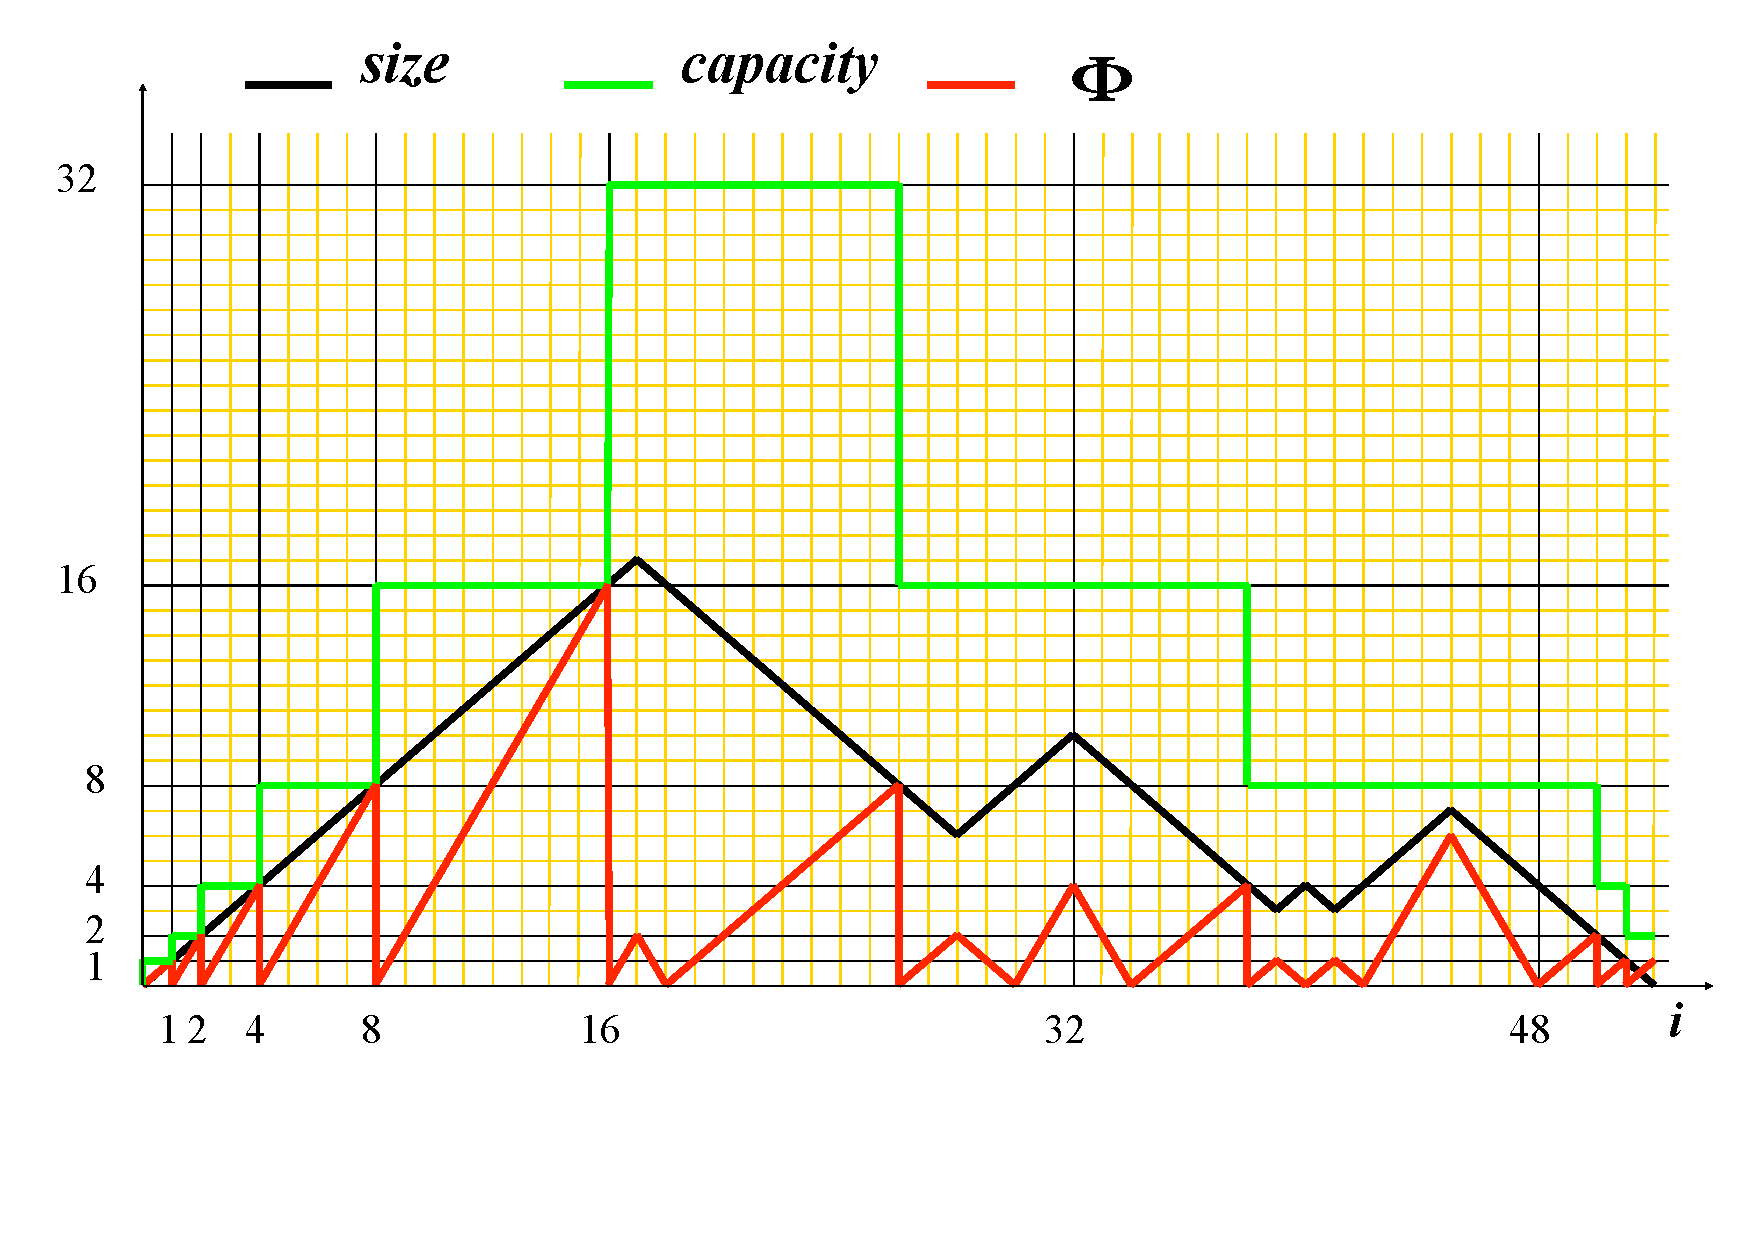
\includegraphics{dynvector.pdf}
\end{frame}

\begin{frame}[shrink]{Vettori dinamici: contrazione}

Se \alert{$\alpha \geq \frac{1}{2}$} il costo ammortizzato di un inserimento \alert{senza espansione} è: 
{\small
\begin{eqnarray*}
a_i &=& c_i + \Phi_i - \Phi_{i-1} \\
    &=& 1 + ( 2 \cdot \textit{dim}_i - \textit{capacità}_i) - ( 2 \cdot \textit{dim}_{i-1} - \textit{capacità}_{i-1})\\
    &=& 1 +  2 \cdot (\textit{dim}_{i-1}+1) - \textit{capacità}_{i-1} -  2 \cdot \textit{dim}_{i-1} + \textit{capacità}_{i-1}\\
    &=& 3
\end{eqnarray*}
}

Se \alert{$\alpha = 1$} il costo ammortizzato di un inserimento \alert{con espansione} è: 
{\small
\begin{eqnarray*}
a_i &=& c_i + \Phi_i - \Phi_{i-1} \\
    &=& 1 + \alert{\textit{dim}_{i-1}} + ( 2 \cdot \textit{dim}_i - \textit{capacità}_i) - ( 2 \cdot \textit{dim}_{i-1} - \textit{capacità}_{i-1})\\
    &=& 1 + \alert{\textit{dim}_{i-1}} +  2 \cdot (\textit{dim}_{i-1}+1) - 2 \cdot \textit{dim}_{i-1} -  2 \cdot \textit{dim}_{i-1} + \textit{dim}_{i-1}\\
    &=& 3
\end{eqnarray*}
}
[ \emph{Esercizio: Altri casi per valori differenti di $\alpha$ e per contrazione} ]
\end{frame}

\section{Conclusioni}

\begin{frame}{Conclusioni}
\BB{Esempi di applicazione dell'analisi ammortizzata}
\BIL
\item Espansione / contrazione di tabelle hash
\item Insiemi disgiunti con euristica sul rango e compressione dei cammini
\item Heap di Fibonacci
\item \ldots
\EIL
	
\end{frame}

\subsection{Reality check}


%% 2020 Spostato in analisi ammortizzata perché fatto dopo
\begin{frame}{Ristrutturazione in tabelle Hash}

\vspace{-9pt}
\BIL
\item Non è conveniente che $\alpha$ cresca troppo
	\BI
	\item In particolare con la scansione interna
	\item Ma vale anche per le liste di trabocco
	\EI
\item Sopra una soglia $t_\alpha$ prefissata (tipicamente $0.5$-$0.75$)
\BI
\item  Si alloca una nuova tabella di dimensione $2m$
\item Si reinseriscono tutte le chiavi presenti nella nuova tabella
\EI
\item Risultato
\BI
	\item Fattore di carico dimezzato (tipicamente $0.25$)
	\item Nessun elemento \textbf{deleted}
\EI
\item Costi
\BI
\item Costo $O(m)$ per la ristrutturazione nel caso pessimo
\item Costo ammortizzato costante (vedi dimostrazione per vettori)
\EI
\EIL

\end{frame}

\begin{frame}[shrink=10]{Reality check}

{\renewcommand*{\arraystretch}{1.4}
\begin{tabular}{|P{2.5cm}|P{4.0cm}|P{0.6cm}|P{4.3cm}|}
\hline
\textbf{Linguaggio} & \textbf{Tecnica} & $t_\alpha$ & \textbf{Note} 
\\ \hline
%
Java 7\newline \texttt{HashMap} &
Liste di trabocco basate su \texttt{LinkedList} &
$0.75$ &
$O(n)$ nel caso pessimo \newline
Overhead: $16n + 4m$ byte
\\ \hline
%
Java 8\newline \texttt{HashMap} &
Liste di trabocco basate su RB Tree &
$0.75$ &
$O(\log n)$ nel caso pessimo \newline
Overhead: $48n + 4m$ byte
\\ \hline
C++ \newline \texttt{sparse\_hash} &
Ind. aperto, scansione quadratica & 
? &
Overhead: $2n$ bit
\\ \hline
C++ \newline \texttt{dense\_hash} &
Ind. aperto, scansione quadratica & 
$0.5$ &
$X$ byte per chiave-valore $\Rightarrow$ 2-3$X$ overhead
\\ \hline
C++ STL \newline \texttt{unordered\_map} &
Liste di trabocco basate su liste &
$1.00$ &
MurmurHash
\\ \hline
Python &
Indirizzam. aperto, scansione quadratica &
$0.66$ &
\\ \hline
\end{tabular}
}
\end{frame}



\end{document}



